Clearly, \gls{idpcdu}'s primary goal is to locate the minimally costly path. Therefore, to accelerate the search process and reduce resource consumption as well as computation time, a pre-filtering process, based on~\cite{binh2021two}, is applied to the input graph $G$ as follows. Firstly, we prune all edges that enter the source node $s$ and leave the target node $t$. Secondly, let $D^k_{i,j}$ be the set of $k$-colored edges going from node $i$ to $j$. If the length of $D^k_{i,j}$ is greater than one, we preserve only the lowest-weight edge and remove the remaining ones in $D^k_{i,j}$. Finally, apart from the source $s$ and target $t$, any node whose indegree and outdegree is 0, is likewise eliminated from $V$. Figure~\ref{fig:filtered_graph} demonstrates $G'=(E', V')$ as a result after performing the pre-filtering process on the input graph.

\setlength{\intextsep}{3pt}
\renewcommand{\scalefigure}{0.8}
\begin{figure}[htbp]
	\centering
	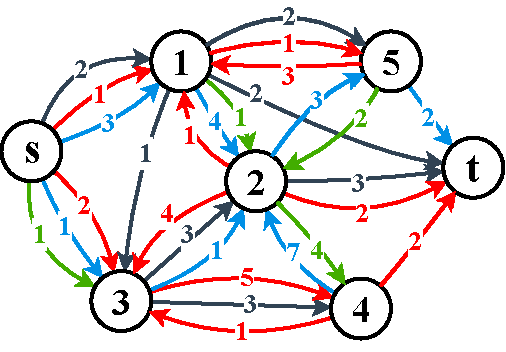
\includegraphics[scale=\scalefigure]{Figures/chap 3/Bold Filtered Graph.pdf}
	\caption{The filtered graph $G'$}
	\label{fig:filtered_graph}
\end{figure}